\begin{introduction}
    \item $Banach$空间~\ref{Banach}
    \item 有界变差函数~\ref{bounded variation}
    \item $L^p$空间~\ref{lp}
    \item $L^{\infty}$空间~\ref{infty}
    \item 赋范线性空间的基~\ref{baseset}
    \item 有限维赋范线性空间~\ref{the:B}
    \item $Riesz$引理~\ref{Riesz}
  \end{introduction}
\section{赋范线性空间概述}
\subsection{范数,赋范线性空间,$Banach$空间} \label{Banach}
在泛函分析中我们大多处理的都是线性的函数空间,这是基于很多函数空间都是无穷维的线性空间这一事实。
无穷维线性空间区别于有限维线性空间,一些在有限维线性空间中成立的事情在无穷维线性空间中不一定成立:
例如,单位闭球在有限维线性空间中是紧致的但在无穷维线性空间中不一定紧致,这点在上一章的讨论中有证明。

在线性代数中,我们定义过$\mathbb{R}^n$上(有限维线性空间)的模长:
\[\mathbb{R}^n \ : \ \vec{v} \in \mathbb{R}^n \ , \ |\vec{v}|=\sqrt{\sum_{i=1}^nx_i^2}\]

在无限维线性空间我们也同样可以定义类似的概念——范数($norm$)可以看作是模长的推广(其实都是距离空间中的距离)。
\begin{definition}[范数]
    设$X$是定义在$\mathbb{R}$或者$\mathbb{C}$上的线性空间,函数$|| \cdot ||:X \to \mathbb{R}$如果满足\\
    \qquad 1. $\forall x \in X \ , \ ||x|| \geq 0 \ \text{and} \ ||x||=0 \ \text{if and only if} \ x=0 \ $(非负性)\\
    \qquad 2. $\forall x \in X \ , \ \forall a \in \mathbb{R} \ or \ \mathbb{C} \ , \ ||ax||=|a|||x|| \ $(齐次性)\\
    \qquad 3. $\forall x,y \in X \ , \ ||x+y|| \leq ||x||+||y|| \ $(三角不等式)\\
    则称$||\cdot||$是$X$上的一个范数,$(X,||\cdot||)$称为赋范线性空间。
\end{definition}
容易证明,赋范线性空间是距离空间。
\begin{definition}[强收敛(依范数收敛)]
    若$d(x_n,x) \to 0 \ (n \to \infty)$即$||x_n-x|| \to 0 \ (n \to \infty)$,则称$x_n$强收敛于$x$或称依范数收敛。
\end{definition}
我们将完备的赋范线性空间称为$Banach$空间。

同一个集合上可以定义不同的范数:
\[(\mathbb{R}^2,|\vec{x}|) \ , \ |\vec{x}|=\sqrt{x_1^2+x_2^2} \qquad \qquad \qquad (\mathbb{R}^2,|\vec{x}|) \ , \ |\vec{x}|=|x_1|+|x_2|\]
\begin{figure}[H]
    \centering
    \begin{minipage}[t]{0.3\textwidth}
    \centering
    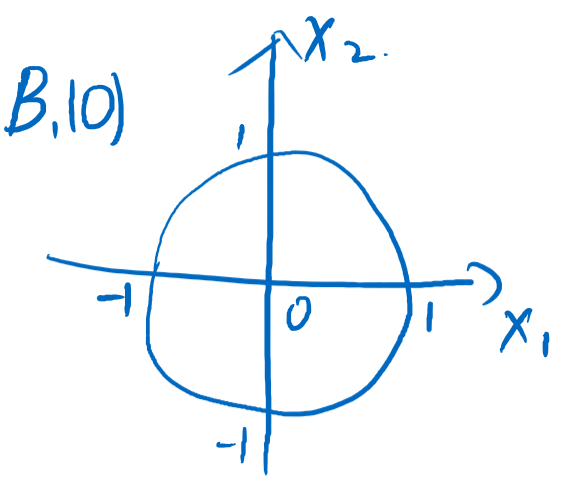
\includegraphics[width=3.5cm]{./fig/3.1.1-1.png}
    \end{minipage}
    \begin{minipage}[t]{0.3\textwidth}
    \centering
    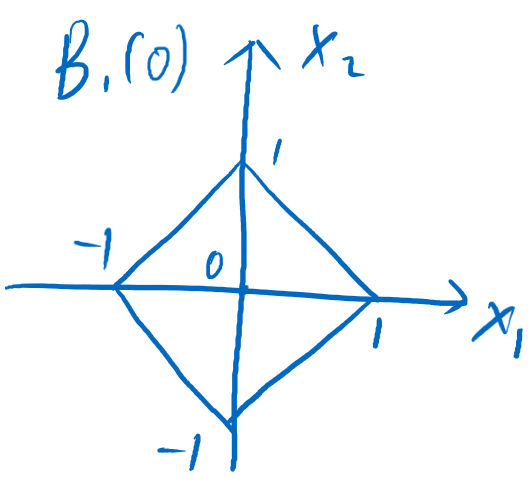
\includegraphics[width=3.5cm]{./fig/3.1.1-2.png}
    \end{minipage}
\end{figure}
下面我们来看几个赋范线性空间的例子。
\paragraph*{例1}$C[a,b] \ , \ ||x(t)||=\mathop \text{sup}\limits_{t \in [a,b]}|x(t)|$是$Banach$空间,无穷维且可分。\\
验证:
\[||x(t)|| \leq 0 \ , \ \text{若}||x(t)||=0 \ \Rightarrow \ \mathop \text{sup}\limits_{t \in [a,b]}|x(t)|=0 \ \Leftrightarrow \ \forall t \in [a,b] \ , \ |x(t)|=0 \ \Rightarrow \ x(t)=0\]
\[||ax(t)||=\mathop \text{sup}\limits_{t \in [a,b]}|ax(t)|=\mathop \text{sup}\limits_{t \in [a,b]}|a||x(t)|=|a|||x(t)||\]
\[||x(t)+y(t)||=\mathop \text{sup}\limits_{t \in [a,b]}|x(t)+y(t)| \leq \mathop \text{sup}\limits_{t \in [a,b]}|x(t)|+\mathop \text{sup}\limits_{t \in [a,b]}|y(t)|=||x(t)||+||y(t)||\]

\paragraph*{例2}$l^{\infty}$是所有有界数列构成的集合,设$X=(x_1,x_2,\cdots)$,设$||X||=\mathop \text{sup}\limits_{i \in \mathbb{N}_+}|x_i|$。容易验证:\\
1、$||\cdot||$是范数; \quad 2、$(l^{\infty},||\cdot||)$是$Banach$空间,无穷维且不可分。

\paragraph*{例3}$L^1[a,b]$是$[a,b]$上所有可积函数(等价类)构成的集合($Lebesgue$积分无法得到严格的相等,只能用等价类来表示,例如若$f=g \ a.e.$,则认为$f$与$g$在$L^1[a,b]$中相同),定义范数
\[||x(t)||_{L^1[a,b]}=\int_a^b|x(t)|\dd t \quad (Lebesgue\text{积分})\]
验证:
\[||x(t)||_{L^1[a,b]}=\int_a^b|x(t)|\dd t \geq 0 \ \text{若}||x(t)||_{L^1[a,b]}=0 \ \Rightarrow \ |x(t)|=0 \ a.e. \ \Rightarrow \ x(t)=0 \ a.e.\]
其余两点容易验证,故$L^1[a,b]$是$Banach$空间。

由此联想,我们也容易想到一个不是$Banach$空间的例子:
\paragraph*{例4}$(C^1[a,b],||\cdot||_{L^1[a,b]})$不完备,故不是$Banach$空间。这件事可以通过范数诱导出的距离加以证明:
\[d(x(t),y(t))=\int_a^b|x(t)-y(t)|\dd t\]

\paragraph*{例5}$V[a,b]$是$[a,b]$上的有界变差函数构成的集合,是$Banach$空间。

当然我们需要先知道有界变差函数是什么。
\begin{definition}[全变差,有界变差函数] \label{bounded variation}
    \[\mathop \text{V}\limits_a^b(x(t))=\mathop \text{sup}\limits_p \sum |x(t_{i+1})-x(t_i)|\]
    其中$p$为$[a,b]$上的任意有限划分$a=t_0<t_1<t_2<\cdots<t_n=b$。\\
    若函数$x(t)$满足
    \[\mathop \text{V}\limits_a^b(x(t))<\infty\]
    则称$x(t)$为有界变差函数。
\end{definition}
首先定义$V[a,b]$上的范数:
\[||x(t)||=|x(a)|+\mathop \text{V}\limits_a^b(x(t))\]
验证其是定义良好的范数:\\
正定性:
\[\text{显然} \ ||x(t)|| \geq 0 \ \text{若} \ ||x(t)||=0 \ \Rightarrow \ x(a)=0 \ \text{且} \ \mathop \text{V}\limits_a^b(x(t))=0 \quad \text{取对半划分:} \ \forall t \in [a,b] \ \text{有:}\]
\[|x(a)-x(t)|+|x(t)-x(b)| \leq \mathop \text{V}\limits_a^b(x(t))=0 \ \Rightarrow \ |x(a)-x(t)|=|x(t)-x(b)|=0 \ \Rightarrow \ x(t)=x(a)=0\]
齐次性显然。\\
三角不等式(注意:这里利用了不等式$\text{sup}(A+B) \leq \text{sup}A+\text{sup}B$)
\begin{equation*}
    \begin{aligned}
        ||x(t)+y(t)|| & =|x(a)+y(a)|+\mathop \text{V}\limits_a^b(x(t)+y(t))=|x(a)+y(a)|+\mathop \text{sup}\limits_p \sum|x_{i+1}(t)-x_i(t)+y_{i+1}(t)-y_i(t)| \\
        & \leq |x(a)|+|y(a)|+\mathop \text{sup}\limits_p \sum|x_{i+1}(t)-x_i(t)|+\mathop \text{sup}\limits_p \sum|y_{i+1}(t)-y_i(t)|=||x(t)||+||y(t)||
    \end{aligned}
\end{equation*}
下面验证$V[a,b]$是$Banach$空间。\\
\textbf{Proof:}\\
设$\{x_n\}$是$V[a,b]$中的柯西列。
\[\forall \varepsilon>0 \ , \ \exists \, N>0 \quad \text{s.t.} \quad n,m \geq N \ , \ ||x_m-x_n||<\varepsilon\]
即对$[a,b]$上的任意有限划分$a=t_0<t_1<t_2<\cdots<t_n=b$都有
\[|x_m(a)-x_n(a)|+\mathop \text{sup}\limits_p \sum |x_m(t_{i+1})-x_n(t_{i+1})-x_m(t_i)+x_n(t_i)|<\varepsilon\]
由此可以得出两件事:一、$\{x_n(a)\}_{n=1}^{\infty}$是柯西列;二、类似的取对半划分:$ \ \forall t \in [a,b] \ $有:
\[|x(a)-x(t)|+|x(t)-x(b)| \leq \mathop \text{V}\limits_a^b(x(t))<\varepsilon \ \Rightarrow \ |x(a)-x(t)|<\varepsilon \ \Rightarrow \ \{x_n(t)-x_n(a)\}_{n=1}^{\infty}\text{是柯西列}\]
有限个柯西列的和还是柯西列,故我们可以得到:$\{x_n(t)\}_{n=1}^{\infty}$是柯西列,即
\[\forall t \in [a,b] \ , \ x_n(t) \xrightarrow{\text{逐点}} x(t)\]
在此基础上,如果我们想进一步证明$x_n(t)$强收敛于$x(t)$,我们需先证明柯西列极限$x(t)$在$V[a,b]$中(利用了有限加和与极限可交换):
\[\mathop \text{V}\limits_a^b(x(t))=x(a)+\mathop \text{sup}\limits_p \lim_{n \to \infty}\sum |x_n(t_{i+1})-x_n(t_i)|=\lim_{n \to \infty} \left ( x_n(a)+\mathop \text{sup}\limits_p \sum |x_n(t_{i+1})-x_n(t_i)| \right )\]
因为$\{x_n(t)\}_{n=1}^{\infty}$是$V[a,b]$中的柯西列,故$\{x_n(t)\}_{n=1}^{\infty}$是$V[a,b]$中的有界集:
\[\forall n \in \mathbb{N}_+ \ , \ \exists \, M>0 \quad \text{s.t.} \quad ||x_n(t)|| \leq M \ \Rightarrow \ \mathop \text{V}\limits_a^b(x(t)) \leq M \ \Leftrightarrow \ \mathop \text{V}\limits_a^b(x(t)) \in V[a,b]\]
下面我们可以开始证明$x_n(t)$强收敛于$x(t)$:
\[||x_n(t)-x(t)||=|x_n(a)-x(a)|+\mathop \text{sup}\limits_p \sum |x_n(t_{i+1})-x(t_{i+1})-x_n(t_i)+x(t_i)|\]
$\exists \, N>0$当$n>N$时:
\[|x_n(a)-x(a)|=\lim_{m \to \infty}|x_n(a)-x_m(a)|<\varepsilon\]
对任意划分$p$:
\[\mathop \text{sup}\limits_p \sum |x_n(t_{i+1})-x(t_{i+1})-x_n(t_i)+x(t_i)|=\lim_{m \to \infty}\mathop \text{sup}\limits_p \sum |x_n(t_{i+1})-x_m(t_{i+1})-x_n(t_i)+x_m(t_i)|\]
\[\leq \lim_{m \to \infty}\mathop \text{sup}\limits_p \sum |x_n(t_{i+1})-x_n(t_i)|+\lim_{m \to \infty}\mathop \text{sup}\limits_p \sum |x_m(t_{i+1})-x_m(t_i)|<\varepsilon+\varepsilon=2\varepsilon\]
\[\Rightarrow \ \forall \varepsilon>0 \ , \ \exists \, N>0 \quad \text{s.t.} \quad n>N \ , \ ||x_n(t)-x(t)||<3\varepsilon \ \Leftrightarrow \ x_n \to x \ (n \to \infty)\]
\textbf{Q.E.D.}

赋范线性空间中一般用$x_n \to x \ (n \to \infty)$表示强收敛。

\subsection{赋范线性空间的基本性质}
下面我们来看一些赋范线性空间的基本性质:
\begin{theorem}
    设$(X,||\cdot||)$是线性赋范空间,则:\\
    1. 范数是连续函数,即$x_n \to x \ \Rightarrow \ ||x_n|| \to ||x|| \ (n \to \infty)$\\
    2. 线性运算是连续映射\\
    i) \ \ $x_n \to x \ , \ y_n \to y \ \Rightarrow \ x_n+y_n \to x+y$\\
    ii) \ $x_n \to x \ , \ a_n \to a \ (\in \mathbb{R} \ or \ \mathbb{C}) \ \Rightarrow \ a_nx_n \to ax$
\end{theorem}
\textbf{Proof}\\
(1):
\[||x_n||=||x_n-x+x|| \leq ||x_n-x||+||x|| \ \Rightarrow \ ||x_n||-||x|| \leq ||x_n-x||\]
\[||x||=||x-x_n+x_n|| \leq ||x-x_n||+||x_n|| \ \Rightarrow \ ||x||-||x_n|| \leq ||x_n-x||\]
\[\Rightarrow \ \text{\Large|} ||x||-||x_n|| \text{\Large|} \leq ||x_n-x|| \to 0 \ (n \to \infty) \ \Rightarrow \ ||x_n|| \to ||x|| \ (n \to \infty)\]
(2.i):
\[||x_n+y_n-x-y|| \leq ||x_n-x||+||y_n-y|| \to 0\]
(2.ii):
\[||a_nx_n-ax|| \leq ||a_nx_n-ax_n+ax_n-ax|| \leq ||a_nx_n-ax_n||+||ax_n-ax||\]
\[=|a_n-a|||x_n||+|a|||x_n-x|| \to 0\]
\textbf{Q.E.D.}

在线性空间中可以利用加法定义级数,赋范线性空间中当然也可以定义级数:
\begin{definition}[级数,部分和,级数收敛]
    设赋范线性空间中的函数列$\{x_n\}_{n=1}^{\infty}$,定义级数为
    \[\sum_{n=1}^{\infty}x_n=x_1+x_2+x_3+\cdots\]
    定义部分和$S_n$
    \[S_n=\sum_{i=1}^nx_i-x_1+x_2+\cdots+x_n\]
    \[\text{若} \ S_n \to S \ (n \to \infty) \ , \ \text{则称级数} \ \sum_{n=1}^{\infty}x_n \ \text{收敛}\]
\end{definition}
\begin{theorem}
    \[(X,||\cdot||) \ \text{是$Banach$空间,级数} \ \sum_{n=1}^{\infty}||x_n|| \ \text{收敛,则} \ \sum_{n=1}^{\infty}x_n \ \text{收敛且} \ \left\| \sum_{n=1}^{\infty}x_n \right\| \leq \sum_{n=1}^{\infty}||x_n||\]
\end{theorem}
\textbf{Proof:}
\[\text{部分和的模长} \ ||S_j||=\left\| \sum_{n=1}^jx_n \right\| \leq \sum_{n=1}^j||x_n||\]
\[\text{由} \ \sum_{n=1}^{\infty}||x_n|| \ \text{收敛} \ \Leftrightarrow \ \forall \varepsilon>0 \ , \ \exists \, N>0 \quad \text{s.t.} \quad j>i \geq N \ , \ \sum_{n=i}^j||x_n||<\varepsilon\]
\[\Rightarrow \ ||S_{j+1}-S_{i-1}||=\sum_{n=i}^j||x_n||<\varepsilon\]
可知部分和序列$\{S_n\}_{n=1}^{\infty}$是柯西列,即$\exists \, S \in X \quad \text{s.t.} \quad S_n \to S \ (n \to \infty)$
\[\text{即} \ \sum_{n=1}^{\infty}x_n \ \text{收敛}\]
进而,由范数$||\cdot||$的连续性,对不等式两边取极限即证毕。
\[\left\| \sum_{n=1}^jx_n \right\| \leq \sum_{n=1}^j||x_n|| \ \Rightarrow \ \left\| \sum_{n=1}^{\infty}x_n \right\| \leq \sum_{n=1}^{\infty}||x_n||\]
\textbf{Q.E.D.}

我们也可以看看赋范线性空间下凸集的性质。
\begin{definition}[凸集]
    设$X$是线性空间,集合$A$满足
    \[A \subset X \ , \ \forall x,y \in A \ , \ t \in (0,1) \quad \text{s.t.} \quad tx+(1-t)y \in A\]
    则称$A$为凸集。
\end{definition}
几何直观:
\begin{figure}[htbp]
    \center
    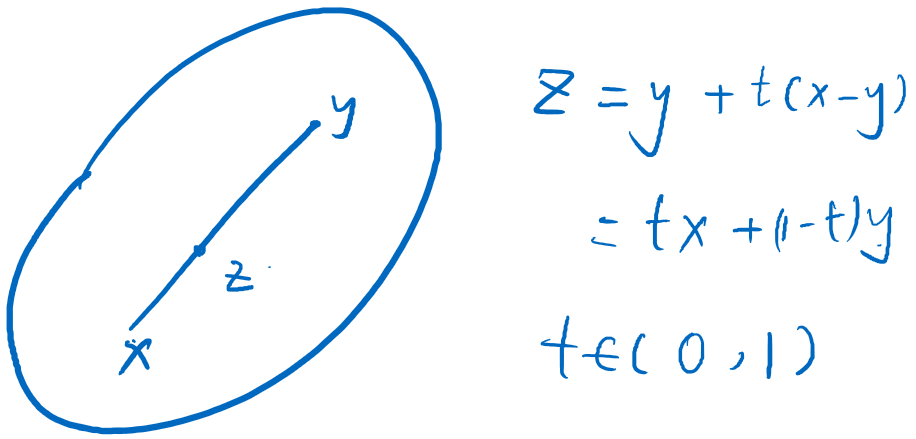
\includegraphics[scale=0.22]{./fig/3.1.2.png}
\end{figure}
\begin{theorem}
    设$(X,||\cdot||)$是赋范线性空间,原点的球邻域$B_r(0)$是凸集。
\end{theorem}
\textbf{Proof:} $B_r(0)=\{x|x \in X \ ,||x||<r\}$,设$x,y \in B_r(0) \ , \ t \in (0,1)$
\[||tx+(1-t)y|| \leq ||tx||+||(1-t)y||=|t|||x||+|1-t|||y||<tr+(1-t)r=r \ \Rightarrow \ tx+(1-t)y \in B_r(0)\]
\textbf{Q.E.D.}
\begin{proposition}
    $(X,||\cdot||)$中任意球是凸集。
\end{proposition}
凸集还有其他基本性质,如任意个凸集的交集是凸集,具体的例子就是赋范线性空间中任意个球的交集是凸集。

关于凸集的性质也有与不动点定理相关的,下面我们简要叙述一下该定理。
\begin{theorem}[$Schauder$不动点定理]
    设$X$是$Banach$空间,$A \subset X$是紧凸集,$T:A \to A$是连续映射,则$T$有不动点(不一定唯一,例如恒等映射)。
\end{theorem}
\paragraph*{例} \quad $T:[0,1] \to [0,1]$
\begin{figure}[htbp]
    \center
    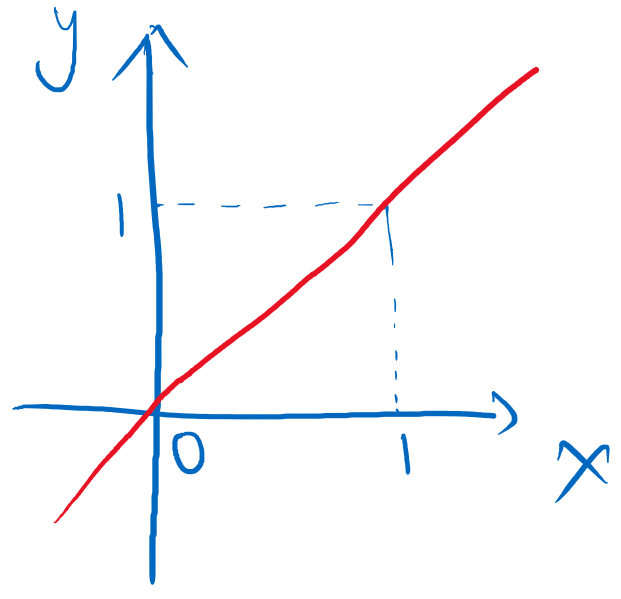
\includegraphics[scale=0.2]{./fig/3.1.2-1.png}
\end{figure}
不动点在$y=x$上,连续映射保证了任意一个$T$都必然与$y=x$有交点。

下面我们将要详细讨论一个赋范线性空间的例子:$L^p(E)$空间 $(p \geq 1)$。

\section{$L^p$空间} \label{lp}
出于方便,我们讨论$L^p$空间的时候都假设$E$是$\mathbb{R}$上的可测集。$L^p$空间定义为
\[L^p(E)=\left\{x(t) \ \text{可测} \ , \ \int_E|x(t)|^p<+\infty\right\}\]
这里$x(t)$是等价类,为方便书写取一代表元,这里$x(t) \sim y(t)$当且仅当$x(t)=y(t) \ a.e. \quad (t \in E)$,在这个集合上我们定义范数:
\[||x(t)||_{L^p(E)}=\left(\int_E|x(t)|^p\dd t\right)^{\frac{1}{p}}\]
验证:\\
\textbf{1、正定性}
\[||x(t)|| \geq 0 \ \text{显然,若}||x(t)||=0 \ \Rightarrow \ \int_E|x(t)|^p\dd t=0 \ \text{,不妨设} \ mE>0 \ \Rightarrow \ x(t)=0 \ a.e.\]
\textbf{2、齐次性}
\[||kx(t)||=\left(\int_Ek|x(t)|^p\dd t\right)^{\frac{1}{p}}=\left(|k|^p\int_E|x(t)|^p\dd t\right)^{\frac{1}{p}}=|k|\left(\int_E|x(t)|^p\dd t\right)^{\frac{1}{p}}\]
\textbf{3、三角不等式}: $Minkowski$不等式\\
要证明上述不等式,我们需要一些其他的基础不等式:
\begin{theorem}[$Young$不等式]
    \[\text{若} \forall p,q>0 \ \text{满足} \ \frac{1}{p}+\frac{1}{q}=1 \ \text{,则对} \ \forall a,b>0 \ \text{都有} \ |ab| \leq \frac{|a|^p}{p}+\frac{|b|^q}{q}\]
\end{theorem}
\textbf{Proof:}不妨设$a,b>0$
\[\frac{1}{p}+\frac{1}{q}=1 \ \Leftrightarrow \ \frac{q}{p}+1=q \ \Leftrightarrow \ 1-q=-\frac{q}{p}\]
\[|ab| \leq \frac{|a|^p}{p}+\frac{|b|^q}{q} \ \Leftrightarrow \ ab^{1-q} \leq \frac{1}{p}\left(\frac{a^p}{b^q}\right)+\frac{1}{q} \ \Leftrightarrow \ \left(\frac{a^p}{b^q}\right)^{\frac{1}{p}}-1 \leq \frac{1}{p}\left(\frac{a^p}{b^q}-1\right)\]
令$t=a^p/b^q>0$,则只需证
\[t^{\frac{1}{p}}-1 \leq \frac{1}{p}(t-1) \quad (t>0 \ ,p>0)\]
令
\[f(t)=t^{\frac{1}{p}}-\frac{1}{p}t-1+\frac{1}{p} \quad (t>0 \ ,p>0)\]
则
\[f'(t)=\frac{1}{p}t^{\frac{1}{p}-1}-\frac{1}{p}=\frac{1}{p}\left(t^{\frac{1}{p}-1}-1\right)\]
易证明$x=1$为$f(x)$的极大值点:
\[f(x) \leq f(1)=0 \ \Rightarrow \ t^{\frac{1}{p}}-1 \leq \frac{1}{p}(t-1) \quad (t>0 \ ,p>0)\]
原命题得证。

\textbf{Q.E.D.}

在使用$Young$不等式的时候我们可以用到一下小技巧:
\[\text{若} \forall p,q>0 \ \text{满足} \ \frac{1}{p}+\frac{1}{q}=1 \ \text{,则对} \ \forall a,b>0 \ , \ \forall \varepsilon>0 \ \text{都有} \ |ab|=|\varepsilon a \cdot \frac{1}{\varepsilon}b| \leq \varepsilon^p\frac{|a|^p}{p}+\frac{1}{\varepsilon^q}\frac{|b|^q}{q}\]
由于$\varepsilon$的任意性,可以用这种小技巧将一些性质不好的项(我不喜欢的项)压住。
\begin{theorem}[$H\ddot{o}lder$不等式]
    设$E$是可测集,$x(t),y(t)$是$E$上的可测函数,则有
    \[\int_E|x(t)y(t)|\dd t \leq \left(\int_E|x(t)|^p\dd t\right)^{\frac{1}{p}}\left(\int_E|y(t)|^q\dd t\right)^{\frac{1}{q}} \quad (p,q>0 \ , \ \frac{1}{p}+\frac{1}{q}=1)\]
    若$x(t) \in L^p(E) \ , \ y(t) \in L^q(E)$则
    \[\int_E|x(t)y(t)|\dd t \leq ||x(t)||_{L^p(E)}||y(t)||_{L^q(E)}\]
\end{theorem}
\textbf{Proof:}设
\[A=||x(t)||_{L^p(E)}=\left(\int_E|x(t)|^p\dd t\right)^{\frac{1}{p}} \qquad B=||y(t)||_{L^q(E)}=\left(\int_E|y(t)|^q\dd t\right)^{\frac{1}{q}}\]
由$Young$不等式:
\[\frac{|x(t)| \cdot |y(t)|}{A \cdot B} \leq \frac{1}{p}\frac{|x(t)|^p}{A^p}+\frac{1}{q}\frac{|y(t)|^q}{B^q} \ \Rightarrow \ \frac{\int_E|x(t)y(t)|\dd t}{A \cdot B} \leq \frac{1}{p}\frac{\int_E|x(t)|^p\dd t}{A^p}+\frac{1}{q}\frac{\int_E|y(t)|^q\dd t}{B^q}=1\]
\[\Rightarrow \ \int_E|x(t)y(t)|\dd t \leq A \cdot B\]

\textbf{Q.E.D.}

下面我可以来证明$Minkowski$不等式($L^p$空间的三角不等式):
\begin{theorem}[$Minkowski$不等式]
    设$x(t),y(t) \in L^p(E) \ (p \geq 1)$,则有
    \[\left(\int_E|x(t)+y(t)|^p\dd t\right)^{\frac{1}{p}} \leq \left(\int_E|x(t)|^p\dd t\right)^{\frac{1}{p}}+\left(\int_E|y(t)|^p\dd t\right)^{\frac{1}{p}}\]
    即
    \[||x(t)+y(t)||_{L^p(E)} \leq ||x(t)||_{L^p(E)}+||y(t)||_{L^p(E)}\]
\end{theorem}
\textbf{Proof:} $p=1$时,显然;$p>1$时,有
\[\frac{1}{p}+\frac{1}{q}=1 \ \Leftrightarrow \ p=(p-1)q\]
由$H\ddot{o}lder$不等式:
\[\int_E|x(t)+y(t)|^p\dd t=\int_E|x(t)+y(t)||x(t)+y(t)|^{p-1}\dd t\]
\[\leq \int_E|x(t)||x(t)+y(t)|^{p-1}\dd t+\int_E|y(t)||x(t)+y(t)|^{p-1}\dd t\]
\[\leq \left(\int_E|x(t)|^p\dd t\right)^{\frac{1}{p}}\left(\int_E|x(t)+y(t)|^{q(p-1)}\dd t\right)^{\frac{1}{q}}+\left(\int_E|y(t)|^p\dd t\right)^{\frac{1}{p}}\left(\int_E|x(t)+y(t)|^{q(p-1)}\dd t\right)^{\frac{1}{q}}\]
\[\leq \left(\int_E|x(t)|^p\dd t\right)^{\frac{1}{p}}\left(\int_E|x(t)+y(t)|^{p}\dd t\right)^{1-\frac{1}{p}}+\left(\int_E|y(t)|^p\dd t\right)^{\frac{1}{p}}\left(\int_E|x(t)+y(t)|^{p}\dd t\right)^{1-\frac{1}{p}}\]
\[\Rightarrow \ \left(\int_E|x(t)+y(t)|^p\dd t\right) \cdot \left(\int_E|x(t)+y(t)|^{p}\dd t\right)^{\frac{1}{p}-1} \leq \left(\int_E|x(t)|^p\dd t\right)^{\frac{1}{p}}+\left(\int_E|y(t)|^p\dd t\right)^{\frac{1}{p}}\]
\[\Leftrightarrow \ \left(\int_E|x(t)+y(t)|^{p}\dd t\right)^{\frac{1}{p}} \leq \left(\int_E|x(t)|^p\dd t\right)^{\frac{1}{p}}+\left(\int_E|y(t)|^p\dd t\right)^{\frac{1}{p}}\]

\textbf{Q.E.D.}

\section{$L^p$空间的性质}
\begin{theorem}[$Riesz-Fischer$定理]
    $L^p(E) \ (p \geq 1)$是$Banach$空间。\footnote{这里我们指定$E$是$\mathbb{R}$上的可测集,因为说明这种情况比较简单(懒}
\end{theorem}
\textbf{Proof:} \\
(想法是通过$L^p$中的收敛控制$L^1$的收敛($H\ddot{o}lder$不等式),进而得到柯西列收敛从而证明完备性)
\[\text{设} \ \{x_n(t)\} \ \text{是} \ L^p(E) \ \text{中的柯西列,取子列} \ \{x_{n_k}(t)\} \ \text{满足} \ ||x_{n_{k+l}}-x_{n_k}||<\frac{1}{2^k} \ (k=1,2,3,\cdots)\]
(做法是
\[\forall k,m>0 \ , \ \exists \, n_k>0 \quad \text{s.t.} \quad n_{k}>n_{k-1} \ , \ ||x_{n_k+m}-x_{n_k}||<\frac{1}{2^k} \ \Rightarrow \ \text{子列} \ \{x_{n_k}(t)\} \ \text{满足要求}\]
)\\
在下面的讨论中我们需要用到$m(E)<+\infty$这个条件,但是这并不是总能满足的,所有我们取可测集$E_1 \subset E \ , \ m(E_1)<+\infty$,由$H\ddot{o}lder$不等式:
\begin{equation*}
    \begin{aligned}
        \int_{E_1}|x_{n_{k+1}}(t)-x_{n_k}(t)|\dd t & \leq \left(\int_{E_1}1^q\dd t\right)^{\frac{1}{q}}\left(\int_{E_1}|x_{n_{k+1}}(t)-x_{n_k}(t)|^p\right)^{\frac{1}{p}} \\
        & \leq \left[m(E_1)\right]^{\frac{1}{q}}||x_{n_{k+1}}(t)-x_{n_k}(t)||_{L^p(E_1)} \leq \left[m(E_1)\right]^{\frac{1}{q}}\frac{1}{2^k}
    \end{aligned}
\end{equation*}
由$Fatou$引理:
\[\Rightarrow \ \int_{E_1} \lim_{n \to \infty}\sum_{k=1}^n|x_{n_{k+1}}(t)-x_{n_k}(t)|\dd t \leq \lim_{n \to \infty} \int_{E_1} \sum_{k=1}^n|x_{n_{k+1}}(t)-x_{n_k}(t)|\dd t \leq \left[m(E_1)\right]^{\frac{1}{q}}\sum_{k=1}^{\infty}\frac{1}{2^k}<\infty\]
\[\Rightarrow \ \sum_{k=1}^{\infty}|x_{n_{k+1}}(t)-x_{n_k}(t)| \ \text{在} \ E_1 \ \text{上} \ a.e. \ \text{收敛}\]
我们知道以下两个事实:1、$E$可以写成可数个有限测度的子集的并集;2、由可列可加性保证可数个零测集的并集还是零测集。
\[\Rightarrow \ \sum_{k=1}^{\infty}|x_{n_{k+1}}(t)-x_{n_k}(t)| \ \text{在} \ E \ \text{上} \ a.e. \ \text{收敛}\]
\[\Rightarrow \ x_{n_l}(t)=x_{n_1}(t)+\sum_{k=1}^{l-1}\left(x_{n_{k+1}}(t)-x_{n_k}(t)\right) \leq x_{n_1}(t)+\sum_{k=1}^{l-1}|x_{n_{k+1}}(t)-x_{n_k}(t)| \ \text{在} \ E \ \text{上} \ a.e. \ \text{收敛}\]

记$x_{n_l}(t)$极限为$x(t)$,柯西列得到的是逐点收敛,为了证明完备性,下面要证明的自然是$x(t) \in L^p(E)$且$x_{n_l}(t) \to x(t) \ (l \to \infty)$,由$Fatou$引理(也可以用控制收敛定理)及柯西列的有界性:
\[\int_E|x(t)|^p\dd t=\int_E\lim_{l \to \infty}|x_{n_l}(t)|^p\dd t \leq \lim_{l \to \infty}\int_E|x_{n_l}(t)|^p\dd t=\lim_{l \to \infty}||X_{n_l}(t)||^p_{L^p(E)}<+\infty\]
即$x(t) \in L^p(E)$。
\begin{equation*}
    \begin{aligned}
        ||x_{n_k}(t)-x(t)||^p_{L^p(E)} & =\int_E|x_{n_k}(t)-x(t)|^p\dd t=\int_E\lim_{l \to \infty}|x_{n_k}(t)-x_{n_l}(t)|^p\dd t \\
        & \leq \lim_{l \to \infty}\int_E|x_{n_k}(t)-x_{n_l}(t)|^p\dd t=\lim_{l \to \infty}||x_{n_k}(t)-x_{n_l}(t)||^p_{L^p(E)} \leq \left(\frac{1}{2^k}\right)^p \to 0 \ (k \to \infty)
    \end{aligned}
\end{equation*}
即$x_{n_k}(t) \to x(t) \ (k \to \infty)$

\textbf{Q.E.D.}
\begin{theorem}
    $L^p(E) \ (p \geq 1)$是可分的。
\end{theorem}
\textbf{Proof} (只证明$E=[a,b]$的情形,其他的不太好证):\\
想法:逐步逼近(用$\Leftarrow$表示逼近):
\[L^p \ \Leftarrow \ \text{有界}L^p \ \Leftarrow \ \text{连续函数} \ \Leftarrow \ \text{多项式} \ \Leftarrow \ \text{有理多项式}\]
(i) 设$x(t) \in L^p(E)$,令
\[x_n(t)=\left \{
\begin{array}{ll}
    x(t) & , \ |x(t)| \leq n \\ 0 & , \ |x(t)|>n
\end{array}
\right.
\]
\[\int_E|x(t)|^p\dd t=\sum_{n=1}^{\infty} \ \int\limits_{E \cap \{n<|x(t)| \leq n+1\}}|x(t)|^p\dd t<\infty\]
\[\Rightarrow \ \forall \varepsilon>0 \ , \ \exists \, N>0 \quad \text{s.t.} \quad n \geq N \ , \ \int\limits_{E \cap \{|x(t)|>n\}}|x(t)|^p\dd t<\left(\frac{\varepsilon}{3}\right)^p\]
\[\Rightarrow \ ||x_n(t)-x(t)||_{L^p(E)}=\left(\int_E|x_n(t)-x(t)|^p\dd t\right)^{\frac{1}{p}}=\left( \ \int\limits_{E \cap \{|x(t)|>n\}}|x(t)|^p\dd t\right)^{\frac{1}{p}}<\left(\frac{\varepsilon}{3}\right)^{p \cdot \frac{1}{p}}=\frac{\varepsilon}{3}\]
(ii) 取定一个$n \geq N$,由$Lusin$定理:
\[\exists \, y(t) \in C[a,b] \ , \ \mathop \text{sup}\limits_{t \in [a,b]}|y(t)| \leq 2n \quad \text{s.t.} \quad m(\{y(t) \neq x(t)\} \cap E)<\left(\frac{\varepsilon}{3}\right)^p \cdot \frac{1}{(3n)^p}\]
\[(\text{可取上述$|y(t)|$的理由:} \ y(t) \in C[a,b] \ \Rightarrow \ \mathop \text{min}\limits_{t \in [a,b]}\{y(t),2n\} \in C[a,b]\]
\[\text{且} \ |x_n(t)| \leq n \ \Rightarrow \ m(\{y(t)=x_n(t)\})\text{不受影响})\]
\[\Rightarrow \ ||x_n(t)-y(t)||_{L^p(E)}=\left(\int_E|x_n(t)-y(t)|^p\dd t\right)^{\frac{1}{p}}=\left( \ \int\limits_{E \cap \{x_n(t) \neq y(t)\}}|x_n(t)-y(t)|^p\dd t\right)^{\frac{1}{p}}\]
\[\leq \left( \ \int\limits_{E \cap \{x_n(t) \neq y(t)\}}(n+2n)^p\dd t\right)^{\frac{1}{p}} \leq \left(\left(\frac{\varepsilon}{3}\right)^p \cdot \frac{1}{(3n)^p} \cdot (3n)^p\right)^{\frac{1}{p}}=\frac{\varepsilon}{3}\]
(iii) 由$Weierstrass$定理,存在有理系数多项式$P(t)$使得
\[\mathop \text{sup}\limits_{t \in [a,b]}|P(t)-y(t)|<\frac{\varepsilon}{3m(E)^{\frac{1}{p}}}\]
\[||P(t)-y(t)||_{L^p(E)}=\left(\int_E|P(t)-y(t)|^p\dd t\right)^{\frac{1}{p}} \leq \left(m(E) \cdot \frac{\varepsilon^p}{3^pm(E)}\right)^{\frac{1}{p}}=\frac{\varepsilon}{3}\]
由三角不等式
\[||P(t)-x(t)||_{L^p(E)} \leq ||P(t)-y(t)||_{L^p(E)}+||y(t)-x_n(t)||_{L^p(E)}+||x_n(t)-x(t)||_{L^p(E)}<\varepsilon\]
由$\varepsilon$的任意性,得$||P(t)-x(t)||_{L^p(E)} \to 0$。即有理多项式集合在$L^p(E)$中稠密,即$L^p(E)$可分。

\textbf{Q.E.D.}

在这$Riesz-Fischer$定理的证明中,我们有提到过不同范数之间的强弱,我们下面对这件事进行以下严格地叙述。

设$m(E)<\infty \ , \ p_1<p_2$,由$H\ddot{o}lder$不等式:
\[\left(\int_E|x(t)|^{p_1}\dd t\right)^{\frac{1}{p_1}} \leq \left[\left(\int_E\left(|x(t)|^{p_1}\right)^{\frac{p_2}{p_1}}\dd t\right)^{\frac{p_1}{p_2}}\left(\int_E1^{\frac{p_2}{p_2-p_1}}\dd t\right)^{1-\frac{p_1}{q_2}}\right]^{\frac{1}{p_1}} \leq \left(\int_E|x(t)|^{p_2}\dd t\right)^{\frac{1}{p_2}} \cdot m(E)^{\frac{1}{p_1}-\frac{1}{p_2}}\]
\[\text{即} \ x(t) \in L^{p_2}(E) \ \Rightarrow \ x(t) \in L^{p_1}(E) \ , \ \text{即} \ L^{p_2}(E) \subset L^{p_1}(E) \ (p_2>p_1)\]

我们自然会好奇,当上面这个性质当$p \to \infty$时成立吗?下面我们来看看$L^{\infty}(E)$空间。我们先引入一些辅助概念来定义$L^{\infty}(E)$空间。
\begin{definition}[本质有界]
    若存在零测集$E_0 \ , \ m(E_0)=0$使$x(t)$在$E/E_0$上有界,则称$x(t)$在$E$上本质有界($essentially \ bounded$)。
\end{definition}
我们将$L^{\infty}(E)$空间定义为:
\[L^{\infty}(E)=\left\{E\text{上本质有界的可测函数构成的集合}\right\}\]
并且定义$L^{\infty}(E)$范数:
\[||x(t)||_{L^p(E)}=\mathop \text{inf}\limits_{\substack{E_0 \subset E \\ m(E_0)=0}}\mathop \text{sup}\limits_{E/E_0}|x(t)|\]
可以验证$||x(t)||_{L^p(E)}$也是范数。我们可以证明,$||x(t)||_{L^p(E)}<\infty \ \Leftrightarrow \ $本质有界。\\
\textbf{Proof:} 若$x(t)$本质有界,则$\exists \, E_0 \quad \text{s.t.} \quad E/E_0$上$|x(t)|$有界$ \ \Rightarrow \ ||x(t)||_{L^{\infty}(E)}<\infty$。\\
反之,由下确界的性质有:
\[\forall n \in \mathbb{Z}_+ \ , \ \exists \,E_n \subset E \ , \ m(E_n)=0 \quad \text{s.t.} \quad \mathop \text{sup}\limits_{E/E_n}|x(t)|<||x(t)||_{L^{\infty}(E)}+\frac{1}{n}\]
令
\[E_0=\bigcup_{n=1}^{\infty}E_n \ , \ m(E_n)=0 \ \Rightarrow \ m(E_0)=0 \ \Rightarrow \ \mathop \text{sup}\limits_{E/E_0}|x(t)|<||x(t)||_{L^{\infty}(E)}<\infty\]
那么$x(t)$本质有界。\\
\textbf{Q.E.D.}
\begin{definition}[本质上界] \label{infty}
    我们称$||x(t)||_{L^{\infty}} (E)$为$x(t)$在$E$上的本质上界(确实是对$|x(t)|$而言的)。
\end{definition}
这里我们不加证明的叙述一些$L^{\infty}(E)$空间的性质,如果我们限定$m(E)<+\infty$,则$\forall x(t) \in L^{\infty}(E) \ , \ x(t) \in L^p(E) \ (p \geq 1)$,反之则不然,这也即:
\[L^{\infty}(E) \subset \bigcap_{p \geq p_0}L^{p}(E) \ (\forall p_0 \geq 1)\]
但需要注意
\[L^{\infty}(E) \neq \bigcap_{p \geq p_0}L^{p}(E) \ (\forall p_0 \geq 1)\]
同时我们也容易看出来$||x||_{L^p(E)} \leq ||x||_{L^{\infty}(E)}$,毕竟正常$L^p$范数可以看作是对函数值的p次几何平均,而$L^{\infty}$范数只取了极大值。下面我们可以看一个具体的例子:
\paragraph*{例} \quad $x(t)=\ln t \ , \ t \in (0,1]$,可以验证$x(t) \in L^p(0,1] \ (p \geq 1)$但$x(t) \notin L^{\infty}(E)(0,1]$。

下面我们看看其他$L^{\infty}(E)$空间的性质。
\begin{theorem}
    $(L^{\infty}(E),||\cdot||_{L^{\infty}(E)})$是$Banach$空间。
\end{theorem}
\textbf{Proof:}设$\{x_n(t)\}$是柯西列,则
\[\exists \, \{x_{n_{k}}(t)\} \subset \{x_n(t)\} \quad \text{s.t.} \quad \forall k,l \in \mathbb{N} \ , \ ||x_{n_{k+l}}(t)-x_{n_{k}}(t)||<\frac{1}{2^k}\]
\[\Rightarrow \ \exists \, E_{k,l} \ , \ m(E_{k,l})=0 \quad \text{s.t.} \quad \forall k,l \in \mathbb{N} \ , \ |x_{n_{k+l}}(t)-x_{n_{k}}(t)|<\frac{1}{2^k} \ , \ \forall t \in E/E_{k,l}\]
由可列可加性:
\[E_0=\bigcup_{k,l\in \mathbb{N}}E_{k,l} \ \Rightarrow \ m(E_0)=0\]
\[\Rightarrow \ \forall t \in E/E_0 \quad \text{s.t.} \quad \forall k,l \in \mathbb{N} \ , \ |x_{n_{k+l}}(t)-x_{n_{k}}(t)|<\frac{1}{2^k}\]
\[\Rightarrow \ \forall t \in E/E_0 \quad \text{s.t.} \quad \sum_{k=1}^{\infty}|x_{n_{k+1}}(t)-x_{n_{k}}(t)|<\sum_{k=1}^{\infty}\frac{1}{2^k}=1<+\infty\]
\[\Rightarrow \ x(t):=\lim_{k \to \infty}x_{n_k}(t) \quad \forall t \in E/E_0 \quad \text{s.t.} \quad |x(t)|=\left|x_{n_1}(t)+\sum_{k=1}^{\infty}(x_{n_{k+1}}(t)-x_{n_{k}}(t))\right|<+\infty\]
$\Rightarrow \ x_{n_k}(t) \to x(t) \ (k \to \infty)$,即$x_{n_k}(t)$逐点收敛到$x(t)$,证明完逐点收敛后下证依范数收敛。
\[\forall t \in E/E_0 \quad \text{s.t.} \quad |x_{n_{k+l}}(t)-x_{n_{k}}(t)|<\frac{1}{2^k} \ \Rightarrow \ \mathop \text{sup}\limits_{E/E_0}|x_{n_{k+1}}(t)-x_{n_{k}}(t)| \leq \frac{1}{2^k} \ (\forall l=1,2,\cdots)\]
当$l \to \infty$时,
\[\mathop \text{sup}\limits_{E/E_0}|x(t)-x_{n_{k}}(t)| \leq \frac{1}{2^k} \ (\forall l=1,2,\cdots)\]
\[\Rightarrow \ ||x(t)-x_{n_k}(t)||_{L^{\infty}(E)}=\mathop \text{inf}\limits_{\substack{E_0 \subset E \\ m(E_0)=0}} \mathop \text{sup}\limits_{E/E_0}|x(t)-x_{n_{k}}(t)| \leq \frac{1}{2^k} \ (\forall k=1,2,\cdots)\]
令$k \to \infty \ , \ x_{n_k}(t) \to x(t)$即$x_{n_k}(t)$依范数收敛到$x(t)$。\\
\textbf{Q.E.D.}

$L^p$空间也有离散情形下的例子,在$\mathbb{Z}_+$上考虑计数测度$\mu_c$,数列$x=\{\xi_n\}_{n=1}^{\infty}$可视为$\mathbb{Z}_+$的可测函数,他的积分:
\[\int_{\mathbb{Z}_+}|x|^p\dd\mu_c=\sum_{n=1}^{\infty}|\xi_n|^p\]
我们定义:
\[l^p=\{\{\xi_n\}_{n=1}^{\infty} \ , \ \sum_{n=1}^{\infty}|\xi_n|^p<\infty\} \qquad ||x||_{l^p}=\left(\sum_{n=1}^{\infty}|\xi_n|^p\right)^{\frac{1}{p}}\]
当$p=\infty$时
\[l^{\infty}=\{\{\xi_n\}_{n=1}^{\infty} \ , \ \mathop \text{sup}\limits_{n \in \mathbb{Z}_+}|\xi_n|<\infty\} \qquad ||x||_{l^{\infty}}=\mathop \text{sup}\limits_{n \in \mathbb{Z}_+}|\xi_n|\]
可以证明$l^p \ , \ l^{\infty}$是$Banach$空间。
\paragraph*{$L^p \ , \ L^{\infty}$的应用举例——纳什迭代($Nash-Moser \ iteration$)} \quad \\
$\Delta u=fu \ , \ f$是给定函数 $u:\Omega \subset \mathbb{R}^n \to \mathbb{R}$,若$f \in L^q(\Omega)$,则$\exists \, c>0 \quad \text{s.t.} \quad ||u||_{L^{\infty}(\Omega)} \leq ||u||_{L^p(\Omega)}$

\section{赋范线性空间的其他性质}
\subsection{赋范线性空间的子空间与完备化}
设$(X,||\cdot||)$是赋范线性空间,$X_1$是$X$的子空间,$(X_1,||\cdot||)$是赋范线性空间,则称$(X_1,||\cdot||)$是$(X,||\cdot||)$的一个子空间。
\begin{theorem}
    \paragraph*{1.} 赋范线性空间的完备子空间是$Banach$空间;
    \paragraph*{2.} $Banach$空间的闭子空间是$Banach$空间。
\end{theorem}
\paragraph*{例} $l^{\infty}$是$Banach$空间,$||x||=\mathop \text{sup}\limits_{n \in \mathbb{Z}_+}|\xi_n| \ , \ x=\{\xi_n\}$,记$c=l^{\infty}$中的收敛数列的集合。可证明$c$是$Banach$空间。\\
\textbf{Proof:} 只需证明$c$是$l^{\infty}$的闭子空间。

设$x_n=\{\xi_{n,i}\}_{i=1}^{\infty}$是$c$中的收敛点列,设$x_n \to x=\{\xi_i\}_{i=1}^{\infty}$,需证$x \in c$,即证$\{\xi_i\}_{i=1}^{\infty}$是收敛数列。
\[\forall \varepsilon>0 \ , \ \exists \, N>0 \quad \text{s.t.} \quad n \geq N \ , \ ||x_n-x||_{l^{\infty}}<\varepsilon \ \Rightarrow \ \exists \, N>0 \quad \text{s.t.} \quad n \geq N \ , \ \mathop \text{sup}\limits_{i \in \mathbb{Z}_+}|\xi_{n,i}-\xi_i|<\varepsilon\]
由于$\{\xi_{n,i}\}_{i=1}^{\infty}$是收敛点列,故它是柯西列,则有
\[\forall \varepsilon>0 \ , \ \exists \, I_n>0 \quad \text{s.t.} \quad i,j \geq I_n \ , \ |\xi_{n,i}-\xi_{n,j}|<\varepsilon\]
则当$i,j \geq I_n$时,有
\[|\xi_{i}-\xi_{j}| \leq |\xi_{i}-\xi_{n,1}|+|\xi_{n,i}-\xi_{n,j}|+|\xi_{n,j}-\xi_{j}|<3\varepsilon\]
即$x=\{\xi_i\}_{i=1}^{\infty}$是柯西列且是实数列,故$x$收敛,从而$x \in c$。\\
\textbf{Q.E.D.}

在上述子空间的内容中我们用到了完备赋范线性空间($Banach$空间),我们自然就会关心赋范线性空间如何完备化的。

我们知道,赋范线性空间是一个距离空间,距离空间是可以完备化的,那么我们自然就会去思考,这样完备化得到的距离空间还是不是赋范线性空间呢?为此我们需要验证其线性结构(加法,数乘)、范数。
\begin{theorem}
    设$(X,||\cdot||)$是不完备的赋范线性空间,它作为距离空间有完备化$\tilde{X}$,可以证明$\tilde{X}$是$Banach$空间。
\end{theorem}
\paragraph*{recall} \quad 设$\tilde{x}=[\{x_n\}] \in \tilde{X}$是$X$中柯西列的等价类。
\paragraph*{定义加法} \quad $\tilde{x}+\tilde{y}=[\{x_n+y_n\}]$\\
容易验证: 1.柯西列相加还是柯西列; 2.加法的定义与等价类无关。
\paragraph*{定义数乘} \quad $k\tilde{x}=[\{kx_n\}]$\\
容易验证: 1.柯西列数乘后还是柯西列; 2.数乘的定义与等价类无关。
\paragraph*{定义范数}
\[||\tilde{x}||_{\tilde{X}}=\lim_{n \to \infty}||x_n||_X\]
我们需要验证:1.$\{\tilde{x}_n\}$是柯西列; 2.$||\tilde{x}||_{\tilde{X}}$的取值与代表元的选取无关。\\
我们知道,$\{x_n\}_{n=1}^{\infty} \subset X$是柯西列时,可以得到$\{||x_n||\}_{n=1}^{\infty}$是收敛的柯西列。
\[\forall \varepsilon>0 \ , \ \exists \, N>0 \quad \text{s.t.} \quad \forall m>n \geq N \ , \ ||x_n-x_m||<\varepsilon\]
\[\forall \varepsilon>0 \ , \ \exists \, N>0 \quad \text{s.t.} \quad \forall m>n \geq N \ , \ \left|||x_n||-||x_m||\right| \leq ||x_n-x_m||<\varepsilon\]
当$m \to \infty$时,记$x:=x_m \ (m \to \infty)$:
\[\forall \varepsilon>0 \ , \ \exists \, N>0 \quad \text{s.t.} \quad \forall n \geq N \ , \ \left|||x_n||-||x||\right|<\varepsilon\]
1.即证。

我们定义等价类为$x \mapsto \tilde{x}=[\{x,x,\cdots\}]$,则$x$可嵌入$\tilde{x}$中,则
\[||\tilde{x}||_{\tilde{X}}=\lim_{n \to \infty}||x_n||_X=||x||_X\]
两个范数的定义是一致的,2.也证毕。\\
\textbf{Q.E.D.}

\subsection{商空间与乘积空间}
在有限维空间中,商空间的定义如下,我们先定义$V$是定义在数域$\mathbf{K}$上的一个向量空间:
\begin{definition}[商空间]
    商空间$V/A=\{\tilde{x}=x+A\}$,其中$\tilde{x}$是一个等价类,等价关系$\sim$定义如下:$x \sim y$当且仅当$x-y \in A$。
\end{definition}
再者,我们定义商映射$\pi:V \to V/A \ , \ x \mapsto \tilde{x}$,显然,这是个线性映射且是满射。
\[\text{加法:}\tilde{x}+\tilde{y}=\tilde{x+y} \qquad \text{数乘:}k\tilde{x}=\tilde{kx} \ (x,y \in V \ , \ k \in \mathbb{K})\]
注:有限维的子空间都是闭子空间。

可以看到,商空间其实是我们所熟知的平行这个概念的推广,现在这个空间中的跟某个$x$之差属于$A$的元素$\tilde{x}$视作一个等价类,可以说说$\tilde{x}$跟x只差了一个$A$。

下面我们来看无限维的情况:假设X是赋范线性空间,$M$是$X$的闭子空间,在商空间$X/M$中定义范数
\[||\tilde{x}||=\mathop \text{inf}\limits_{y \in \tilde{x}}||y||=\mathop \text{inf}\limits_{y-x \in M}||y||=\mathop \text{inf}\limits_{z \in M}||x+z||\]
则课称$X/M$是关于$M$的赋范商空间。我们可以验证$||\tilde{x}||$是范数:
\paragraph*{1、正定性} \quad $||\tilde{x}||>0$是显然的,而当
\[||\tilde{x}||=0 \ , \ \exists \, \{y_n\}_{n=1}^{\infty} \subset \tilde{x} \quad \text{s.t.} \quad \lim_{n \to \infty}||y_n||=0\]
而由于$M$是闭子空间,$x+M$也是闭子空间,故$\exists \, y \in \tilde{x} \quad \text{s.t.} \quad y_n \to y \ (n \to \infty)$
\[||y||=\lim_{n \to \infty}||y_n||=0 \ \Rightarrow \ y=0 \ \Rightarrow \ \tilde{x}=\tilde{y}=\tilde{0}\]
\paragraph*{2、齐次性}
\[||k\tilde{x}||=\mathop \text{inf}\limits_{y \in k\tilde{x}=\tilde{kx}}||y||=\mathop \text{inf}\limits_{z \in \tilde{x}}||kz||=|k|\mathop \text{inf}\limits_{z \in \tilde{x}}||z||=|k|||\tilde{x}||\] 
\paragraph*{3、三角不等式} \quad $\tilde{x},\tilde{y} \in X/M$
\[||\tilde{x}+\tilde{y}||=\mathop \text{inf}\limits_{z \in \tilde{x+y}}||z||=\mathop \text{inf}\limits_{z \in M}||x+y+z|| \leq \mathop \text{inf}\limits_{z \in M}\left(||x+\frac{1}{2}z||+||y+\frac{1}{2}z||\right)\]
\[\leq \mathop \text{inf}\limits_{z \in M}||x+\frac{1}{2}z||+||y+\mathop \text{inf}\limits_{z \in M}\frac{1}{2}z||=||\tilde{x}||+||\tilde{y}||\]
关于商空间,我们有以下定理。
\begin{theorem}
    若$X$是$Banach$空间,$M$是$X$的闭子空间,那么$X/M$是$Banach$空间。
\end{theorem}
\textbf{Proof:} 设$\{\tilde{x}_n\}$是$X/M$中的柯西列,取其子列$\{\tilde{x}_{n_k}\}$使得$||\tilde{x}_{n_{k+1}}-\tilde{x}_{n_k}||<1/2^k \ (k=1,2,\cdots)$,由范数的定义:
\[\mathop \text{inf}\limits_{y_k \in \tilde{x}_{n_{k+1}}-\tilde{x}_{n_k}}||y_k||<\frac{1}{2^k} \quad (\forall k \in \mathbb{Z}_+) \quad \Leftrightarrow \quad \exists \, y_k \in \tilde{x}_{n_{k+1}}-\tilde{x}_{n_k} \quad \text{s.t.} \quad ||y_k||<\frac{1}{2^k}\]
\[\Rightarrow \quad \sum_{k=1}^{\infty}y_k \ \text{在$X$中收敛} \quad \Rightarrow \quad x_{n+1}+\sum_{k=1}^{\infty}y_k \ \text{在$X$中收敛,记极限为} \ S\]
记上述级数的部分和为$S_i$,则易知$S_i$在$X$中的收敛
\[S_i=x_{n_1}+\sum_{k=1}^{i-1}y_k\]
则
\[\tilde{S}_i=\tilde{x}_{n_1}+\sum_{k=1}^{i-1}\tilde{y}_k=\tilde{x}_{n_1}+\sum_{k=1}^{i-1}\left(\tilde{x}_{n_{k+1}}-\tilde{x}_{n_k}\right)=\tilde{x}_{n_i}\]
\[\Rightarrow \quad ||\tilde{x}_{n_i}-\tilde{x}||=||\tilde{S}_i-\tilde{x}||=\mathop \text{inf}\limits_{y \in \tilde{S}_i-\tilde{x}}||y|| \leq ||S_i-x||\rightarrow 0 \quad (i \rightarrow \infty)\]
子列收敛,故原柯西列也收敛。

\textbf{Q.E.D.}
\begin{definition}[乘积空间]
    设$(X_1,||\cdot||_{X_1})$与$(X_2,||\cdot||_{X_2})$是赋范线性空间,则称$(X_1 \times X_2,||\cdot||)$为乘积空间,其中范数定义如下
    \[||(x_1,x_2)||=||x_1||_{X_1}+||x_2||_{X_2} \quad (\forall x_1 \in X_1,x_2 \in X_2)\]
\end{definition}
若$(X_1,||\cdot||_{X_1})$与$(X_2,||\cdot||_{X_2})$是$Banach$空间,则$(X_1 \times X_2,||\cdot||)$也为$Banach$空间。

\subsection{赋范线性空间的基} \label{baseset}
对有限维赋范线性空间$X$,如果我们称$\{e_i\}_{i=1}^{\infty} \subset X$为是$X$的一组基,则其应满足
\[\forall x \in X \ , \ \exists \, ! (\xi_1,\xi_2,\cdots,\xi_n) \in \mathbb{R}^n \quad \text{s.t.} \quad x=\sum_{i=1}^n\xi_ie_i\]

类似的,我们也希望基的概念能拓展到无限维的赋范线性空间上来\footnote{毕竟泛函分析又名无穷维线性代数(乐},类似的我们可能会有以下两种想法(然而并不会):
\paragraph*{$Hamel$基}
如果我们保留有限组合这个性质,我们按照如下方式可以定义$Hamel$基:
\begin{definition}[$Hamel$基]
    设无穷维赋范线性空间$X$的线性无关子集为$\{x_{\alpha}\} \ (\alpha \in \Lambda)$,若其张成的空间(称为线性包)满足$\text{Span}\{x_{\alpha}\}=X$,则称$\{x_{\alpha}\}$为$X$的一个$Hamel$基。
\end{definition}
这样的基是有限维赋范线性空间的基的直接推广,它总是存在的(这点可以利用$Zorn$引理证明,但这个结果其实挺显然而且我不关心这个证明所以我不证),但缺点也很明显,就是基的个数可能会太多,这显然会给运算带来很大的麻烦。

于是便有了另外一种基的出现:
\paragraph*{$Schauder$基}
我们将组合的个数适当拓展到至多可数,我们便可按照如下方式定义$Schauder$基:
\begin{definition}[$Schauder$基]
    设无穷维赋范线性空间$X$中的点列$\{e_n\}_{n=1^{\infty}}$若满足
    \[\forall x \in X \ , \ \exists \, !\{\xi_n\}_{n=1}^{\infty} \ (\xi_n \in \mathbb{R}^1) \quad \text{s.t.} \quad x=\sum_{i=1}^{\infty}\xi_ie_i\]
    则称$\{e_n\}_{n=1^{\infty}}$是$X$的一个$Schauder$基。
\end{definition}
当然,从定义可以看出,不是所有赋范线性空间都有$Schauder$基,$Schauder$基的存在要求其赋范线性空间是可分的。
\paragraph*{例1} \quad $l^p \ (p \geq 1) \ , \ e_i=\{0,\cdots,0,1,0,\cdots\}$ (第$i$位为1),可验证$\{e_n\}_{n=1}^{\infty}$是$Schauder$基。
\paragraph*{例2} \quad $L^2[0,2\pi]$可验证$\{1,\cos nx,\sin nx \ (n=1,2,\cdots)\}$是$Schauder$基。

对于$Schauder$基还有以下小结论:
\[x=\sum_{i=1}^{\infty}\xi_ie_i=\lim_{n \to \infty}\sum_{i=1}^{n}\xi_ie_i \quad \Leftrightarrow \quad ||x-\sum_{i=1}^n\xi_ie_i||=||\sum_{i=n+1}^{\infty}\xi_ie_i|| \rightarrow 0 \quad (n \rightarrow 0) \quad \Rightarrow \quad \xi_i \rightarrow 0 \ (i \to \infty)\]
该结论可以用于快速判断某些点列是不是$Schauder$基,同时,这其实也暗示了可分的赋范线性空间其实“维数”也并不是很多。
\paragraph*{例1} \quad $l^{\infty} \ , \ e_i=\{0,\cdots,0,1,0,\cdots\}$ (第$i$位为1),$\{e_n\}_{n=1}^{\infty}$不是$Schauder$基。

这是显然的,因为该点列末端并不$\to 0$。
\begin{theorem}
    $Banach$空间$X$有$Schauder$基,则$X$可分。
\end{theorem}
\textbf{Proof:}
\[\text{令}A=\left\{\left.x=\sum_{i=1}^nr_ie_i\right|r_i \in \mathbb{Q} \ , \ n \in \mathbb{N}\right\}\text{,则$A$是可数集}\]
下证$A$在$X$中稠密,即:
\[\forall \varepsilon>0 \ , \ x \in X \ , \ x=\sum_{i=1}^{\infty}\xi_ie_i \quad \Leftrightarrow \quad \lim_{n \to \infty}||x-\sum_{i=1}^n\xi_ie_i||=0 \quad \Leftrightarrow \quad \exists \, N \in \mathbb{N} \quad \text{s.t.} \quad ||x-\sum_{i=1}^N\xi_ie_i||<\frac{\varepsilon}{2}\]
容易看出:
\[\exists \, r_1,r_2,\cdots,r_N \in \mathbb{Q} \ , \ y=\sum_{i=1}^Nr_ie_i \in A \quad \text{s.t.} \quad ||y-\sum_{i=1}^N\xi_ie_i||=||\sum_{i=1}^N(r_i-\xi_i)e_i|| \leq \sum_{i=1}^N|r_i-\xi_i|\cdot||e_i||\]
利用$Schwartz$不等式:
\[\sum_{i=1}^N|r_i-\xi_i|\cdot||e_i|| \leq \sqrt{\sum_{i=1}^N|r_i-\xi_i|^2} \cdot \sqrt{\sum_{i=1}^N||e_i||^2} \leq N \cdot \mathop \text{max}\limits_i||e_i|| \cdot \mathop \text{max}\limits_i|r_i-\xi_i|<\frac{\varepsilon}{2}\]
故有
\[||x-y|| \leq ||x-\sum_{i=1}^N\xi_ie_i||+||y-\sum_{i=1}^N\xi_ie_i||<\varepsilon\]

\textbf{Q.E.D.}

但是反之并不一定成立,可分的$Banach$空间并不一定有$Schauder$基。
\vspace{0.5cm}
同一个空间可以定义不同的范数,也即不同的距离函数,那我们自然而然地会想问不同距离函数之间是否有关系,他们的收敛性如何让,拓扑关系如何?
\begin{definition}[等价范数]
    设$||\cdot||_1,||\cdot||_2$是赋范线性空间$X$上的两个范数,若满足
    \[\forall x \in X \ , \ \exists \, c>0 \quad \text{s.t.} \quad ||x||_1 \leq c||x||_2\]
    则称$||\cdot||_2$比$||\cdot||_1$强。\\
    如果$||\cdot||_1$比$||\cdot||_2$强且$||\cdot||_2$比$||\cdot||_1$强,则称$||\cdot||_2,||\cdot||_1$等价,即
    \[\forall x \in X \ , \ \exists \, c_1,c_2>0 \quad \text{s.t.} \quad c_1||x||_1 \leq ||x||_2 \leq c_2||x||_1\]
\end{definition}
一个范数比一个范数更强,这种说法看起来比较模糊,其实强想描述的事情就是一个范数能被另外一个范数控制:
\begin{theorem}
    $||\cdot||_2$比$||\cdot||_1$强$ \quad \Leftrightarrow \quad \forall \{x_n\}_{n=1}^{\infty} \subset X \ , \ \text{if} \ ||x_n||_2 \to 0 \ , \ ||x_n||_1 \to 0$
\end{theorem}
\textbf{Proof:}\\
$"\Rightarrow" \quad \exists \, c>0 \quad \text{s.t.} \quad 0 \leq ||x_n||_1 \leq c||x_n||_2 \to 0 \quad \Rightarrow \quad ||x_n||_1 \to 0$\\
$"\Leftarrow" \quad$ 反证法,如若不然,则有:$\forall k \in \mathbb{N} \ , \ \exists \, x_k \in X \quad \text{s.t.} \quad ||x_k||_1>k||x_n||_2$\\
\[\text{令} \ y=\frac{x_k}{||x_k||_1} \ , \ \text{则} \ ||y_k||_1=\left\|\frac{x_k}{||x_k||_1}\right\|_1=1>k\frac{||x_k||_2}{||x_k||_1}=k\left\|\frac{x_k}{||x_k||_1}\right\|_2\]
\[\Rightarrow \quad ||y_k||_2<\frac{1}{k} \to 0 \quad (k \to \infty) \ \text{,但} \ ||y_k||_1=1\]
推出矛盾,故原命题成立。

\textbf{Q.E.D.}

\section{有限维赋范线性空间}
我们常常戏称希尔伯特空间是大号欧氏空间,是因为两者具有类似的空间结构和内积定义,加之可数和有限其实没多大差别。
但是在更一般的距离空间中,如果我们还想获得和欧氏空间类似的性质时,我们对空间的要求可以预料到会有相应的提高。
但这样的提高具体的条件是什么呢,看看本小结的标题就知道了。
\begin{theorem}\label{the:B}
    \textbf{1.} \quad 有限维赋范线性空间上的任意两个范数等价;\\
    \textbf{2.} \quad 任意$n$维赋范线性空间$X$与$\mathbb{R}^n$代数同构,拓扑同胚\footnote{代数同构指的是作为线性空间两者同构,可以用一个保持线性结构的双射关联;拓扑同胚指的是两者可以用一个双连续映射关联。}。
\end{theorem}
\textbf{Proof:} \quad 设$X$是$n$维赋范线性空间,$\{e_1,e_2,\cdots,e_n\}$是$X$的基,定义如下映射
\[T: \qquad X \to \mathbb{R}^n \qquad x=\sum_{i=1}^n\xi_ie_i \mapsto \xi=(\xi_1,\xi_2,\cdots,\xi_n)\]
易知$T$是良定义的,且是双射(因为基表示是唯一的),则$X$与$\mathbb{R}^n$线性同构,下证同胚。

考虑范数$||\cdot||_X$和$||x||_T:=||TX||_{\mathbb{R}^n}$,任意验证后者确实是范数。

第一步,通过算子的有界即连续(不知道为什么算子范数的内容会出现在这里)验证$T^{-1}$的连续性。
\[\forall x \in X \ , \ ||x||_X\left\|\sum_{i=1}^n\xi_ie_i\right\| \leq \sum_{i=1}^n|\xi_i|||e_i|| \leq \left(\sum_{i=1}^n|\xi_i|^2\right)^{\frac{1}{2}}\left(\sum_{i=1}^n||e_i||^2\right)^{\frac{1}{2}}:=\alpha||\xi||_{\mathbb{R}^n}\]
\[\Leftrightarrow \quad ||TX||_{\mathbb{R}^n} \geq \frac{1}{\alpha}||x|| \quad \Leftrightarrow \quad ||\xi||_{\mathbb{R}^n} \geq \frac{1}{\alpha}||T^{-1}\xi|| \quad \Rightarrow \quad \alpha \geq ||T^{-1}||\]
然后由$T^{-1}$的有界性知其连续,这个性质的证明等下一章再说。

第二步,同样的方法,利用上一步的结论,考虑函数$f$:
\[f: \qquad \mathbb{R}^n \to \mathbb{R} \qquad \xi \mapsto ||T^{-1}\xi||=||x||\]
容易验证$f$连续,$\forall \xi \eta \in \mathbb{R}^n \ , \ x:=T^{-1}\xi \ , \ y:=T^{-1}\eta$
\[|f(\xi)-f(\eta)|=|||x||-||y||| \leq ||x-y|| \leq \alpha ||T(x-y)||_{\mathbb{R}^n}=\alpha ||\xi-\eta||_{\mathbb{R}^n}\]

由于有限维,$f$限制在单位球面$S^{n-1} \subset \mathbb{R}^n$(紧集)上的最值可被达到,这里考虑最小值,即
\[\exists \, \xi_0=\sum_{i=1}^n\xi_0^ie_i \in S^{n-1} \quad \text{s.t.} \quad \beta:=f(\xi_0)=\mathop \text{min}\limits_{x \in S^{n-1}}f(x)=\left\|\sum_{i=1}^n\xi_0^ie_i\right\|>0\]
记$q=||\xi||_{\mathbb{R}^n}$,则
\[||x||=q\left\|\frac{x}{q}\right\|=qf\left(\frac{\xi}{q}\right) \geq q\beta=\beta||Tx||_{\mathbb{R}^n}\]
同上可知然后由$T$连续。

综上所述,$T$的拓扑同胚可证,最后由于范数$||x||$的任意性可知原命题成立。(实际上证明的是两个范数$||\cdot||_X$和$||x||_T:=||TX||_{\mathbb{R}^n}$等价)

\textbf{Q.E.D.}

上述定理告诉我们有限维的赋范线性空间基本上可以直接当成欧氏空间来看,当然是在范数意义下。
从证明中我们还可以知道,任意有限维赋范线性空间都是完备的,其上点列的依范数收敛直接等价于坐标分量收敛,这点可以通过证明中定义的映射$T$看出。

最重要的,有限维赋范线性空间中的有界集列紧,有界闭集是紧集。这个性质还可以用于判定一个赋范线性空间是否为有限维,我们将在后面证明这个定理,但在证明之前我们需要先介绍一个非常有用的工具——$Riesz$引理。
\begin{theorem}[$Riesz$引理]\label{Riesz}
    设$X_0$是赋范线性空间$X$的真闭子空间(不要求有限维),则
    \[\forall \varepsilon>0 \ , \ \exists \, x_0 \in X / X_0 \quad \text{s.t.} \quad ||x_0||=1 \ , \ d(x_0,X_0):=\mathop \text{inf}\limits_{x \in X_0}d(x_0,x) \geq 1-\varepsilon\]
\end{theorem}
\textbf{Proof:} 依照定理描述,我们知道
\[\forall x_1 \in X/X_0 \ , \ d:=d(x_1,X_0)=\mathop \text{inf}\limits_{x \in X_0}d(x_1,x)=\mathop \text{inf}\limits_{x \in X_0}||x_1-x||\]
由于$X_0$闭,可知$d>0$,且由下确界性质可知
\[\forall \varepsilon \in (0,1) \ , \ \exists \, x_2 \in X_0 \quad \text{s.t.} \quad d(x_1,x_2)=||x_1-x_2||<\frac{d}{1-\varepsilon}\]
则此时我们如下定义$x_0$
\[x_0=\frac{x_1-x_2}{||x_1-x_2||} \quad \Rightarrow \quad ||x_0||=1 \ , \ \forall x \in X_0 \ , \ ||x-x_0||=\left\|x-\frac{x_1-x_2}{||x_1-x_2||}\right\|=\frac{1}{||x_1-x_2||}\left\|||x_1-x_2||x+x_2-x_1\right\|\]
式中$||x_1-x_2||x+x_2 \in X_0$,故
\[\forall x \in X_0 \ , \ ||x-x_0|| \geq \frac{1}{||x_1-x_2||} \cdot d >\frac{1-\varepsilon}{d} \cdot d=1-\varepsilon\]

\textbf{Q.E.D.}

关于$Riesz$引理有很多可以细嗦的东西,但是我们先来看一幅图直观感受一下。
\begin{figure}[H]
    \center
    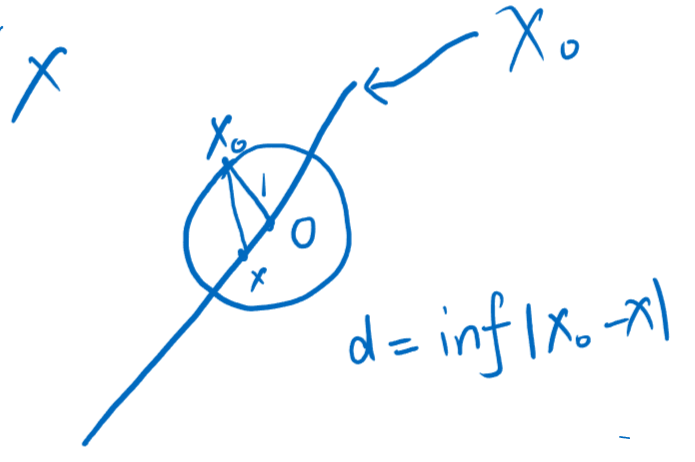
\includegraphics[scale=0.25]{./fig/3.5-1.png}
\end{figure}

对于$d(x_0,X_0)$我们首先应该能想到应该对应于$x_0 \perp X_0$,但是在赋范线性空间我们没办法定义垂直这件事,而$Riesz$引理告诉我们我们能找到一个差不多垂直的元素,当然由于差不多垂直,所以并不能保证$d(x_0,X_0) \geq 1$成立。
但是如果我们在有限维空间中考虑这件事,由完备性可知确实一定存在一个点满足$d(x_0,X_0) \geq 1$,\textbf{所以还是有限维香啊}。
我们可以严格描述并证明上面这句话。

\begin{proposition}
    若$X_0$为有限维真闭子空间,则$\exists \, x_0 \in S \quad \text{s.t.} \quad d(x_0,X_0)=1$。
\end{proposition}
\textbf{Proof:} 
\[\forall y_0 \in X/X_0 \ , \ d:=d(y_0,X_0)>0 \ , \ \exists \, x_0 \in X_0 \quad \text{s.t.} \quad d \leq d(t_0,x_n)<d(y_0,x_0)-\frac{1}{n}\]
通过上述方式构造出的点列$\{x_n\}$满足$||x_n|| \leq ||x_n-y_0||+||y_0||<+\infty$,是有限维闭子空间上的点列,由有限维赋范线性空间的性质可知$\{x_n\}$列紧,不妨设$x_n \to x_0 \in X_0$,其中$x_0$被称为\textbf{最佳逼近元}。
\[d \leq d(y_0,x_n)<d(y_0,x_0)-\frac{1}{n} \ (n \to \+\infty) \quad \Rightarrow \quad d(y_0,x_0)=d\]
取球面上另外一点$x'$满足如下条件可验证$d(x',X_0)=1$。
\[x'=\frac{y_0-x_0}{||y_0-x_0||} \quad \Rightarrow \quad d(x',X_0)=\mathop \text{inf}\limits_{z \in X_0}\left\|\frac{y_0-x_0}{||y_0-x_0||}-z\right\|=\frac{1}{||y_0-x_0||}\mathop \text{inf}\limits_{z \in X_0}\left\|||y_0-x_0||z+x_0-y_0\right\|=\frac{1}{d} \cdot d=1\]

\textbf{Q.E.D.}

顺便严格定义一下最佳逼近元。
\begin{definition}[最佳逼近元]
    设$(X,||\cdot||)$是赋范线性空间,$Y$是$X$的子空间,对$x \in X$,如果
    \[\exists \, y_0 \in Y \quad \text{s.t.} \quad ||x-y_0||=d(x,Y)=\mathop \text{inf}\limits_{y \, \in Y}||x-y||\]
    则称$y_0$为$Y$上关于$X$的最佳逼近元。
\end{definition}

但是在一般的情形下(无限维),最佳逼近元可能不存在,我们可以看下面一个例子。

\paragraph*{例1} \quad 设$X=\left\{f \in C[0,1]|f(0)=0\right\}$,其中$X_0 \in X$为
\[X_0=\left\{f \in X \Big{|} \int_0^1f(x)\dd x=0\right\}\]
则不存在$f \in S \quad \text{s.t.} \quad d(f,X_0)=1$。\\
\textbf{Proof:} \quad 采用反证法,假设$\exists \, f \in S \quad \text{s.t.} \quad d(f,X_0)=1$。
\[f_0 \in X \quad \Rightarrow \quad f_0 \in C[0,1] \ , \ f_0(0)=0 \ , \ ||f_0||=\mathop \text{sup}\limits_{x \in [0,1]}|f(x)|=1 \quad \Rightarrow \quad \left|\int_0^1f_0(x)\dd x\right|<1\]
另一方面
\[\forall f \in X/X_0 \ , \ \exists \, a \in \mathbb{R}^1 \quad \text{s.t.} \quad \int_0^1(f_0-af)\dd x=0 \quad (a=\int_0^1f_0(x)\dd x \Big{/} \int_0^1f(x)\dd x)\]
即$f_0-af \in X_0$,则
\[||f_0-(f_0-af)||=|a|||f|| \geq d(f_0,X_0)=1 \quad \Rightarrow \quad \left|\int_0^1f_0(x)\dd x\right|||f|| \geq \left|\int_0^1f(x)\dd x\right|\]
特别的,我们可以取$f$为一族函数$f_n(x)=x^{1/n}$,则
\[||f_n||=1 \ , \ \left|\int_0^1f_n(x)\dd x\right|=\frac{n}{n+1}\]
进而
\[\left|\int_0^1f_0(x)\dd x\right|||f_n|| \geq \left|\int_0^1f_n(x)\dd x\right|=\frac{n}{n+1} \to 1 \quad (n \to +\infty)\]
得出矛盾。\\
\textbf{Q.E.D.}

同时,即使最佳逼近元存在也可能不唯一,再看一个例子。

\paragraph*{例2} \quad $X=\mathbb{R^2} \ , \ ||\mathbf{x}||=||(x_1,x_2)||=\text{max}\left\{|x_1|,|x_2|\right\}$,取$\mathbf{x}_0=(0,1) \ , \ \mathbf{e}_1=(1,0) \ , \ X_0=\text{span}\{\mathbf{e}_1\}$,
\[\forall \mathbf{y} \in X_0 \ , \ \mathbf{y}=\lambda \mathbf{e}_1=(\lambda,0) \ , \ ||\mathbf{x}_0-\mathbf{y}||\text{max}\left\{|\lambda|,1\right\} \geq 1\]
则可知$\forall ||\mathbf{y}|| \leq 1$都是最佳逼近元。

下面我们就可以开始证明之前提到过的判定赋范线性空间有限维的定理了。

\begin{theorem}
    赋范线性空间$X$为有限维当且仅当$X$中任意有界集都是列紧的。
\end{theorem}
\textbf{Proof:} 一方面,由于$X$与$\mathbb{R}^n$同胚,在$X$上的有界集$E$的像集$T(E)$在$\mathbb{R}^n$有界,而$\mathbb{R}^n$上的有界集$T(E)$列紧,再由同胚可知$X$上的有界集$E$列紧。

另一方面,采用反证法,假设$X$是无穷维,任取$e_1 \in S=\{x \in X | \, ||x||=1\}$,由$Riesz$引理
\[X_1=\text{span}\{e_1\} \ , \ \exists \, e_2 \in S \ , \ d(e_2,X_1)>1-\frac{1}{2}=\frac{1}{2}\]
进而
\[X_2=\text{span}\{e_1,e_2\} \ , \ e_3 \in S \ , \ d(e_3,X_2)>\frac{1}{2} \quad \Rightarrow \quad d(e_3,e_1)>\frac{1}{2} \ , \ d(e_3,e_2)>\frac{1}{2}\]
由反证条件,上述操作可以一直做下去,可以得到序列$\{e_n\} \subset X$满足
\[\forall i,j \in \mathbb{N} \ , \ d(e_i,e_j)>\frac{1}{2} \ , \ ||e_i||=1\]
由于$X$中任意有界集都是列紧的可知$\exists \, \{e_{n_k}\} \subset \{e_i\}$收敛,故矛盾。

\textbf{Q.E.D.}